\section{2019-09-12}
Recall, IP problems are obtained from LP problems by requiring
a non-empty subset of variables to be integers. So, in IP problems
we are allowed to have constraints $x_i\in\mathbb{Z}$, $x\in\mathbb{Z}^n$,
$x_i\in\{0,1\}$, $x_i$ is an integer, $x_i\in\{0,1\}^n$.

\subsection{Example (Assignment Problem)}
SPIT has a campus near the North Pole. They have three buildings named
$A,B,C$ which need to be renovated to be served as one of a
Library, Laboratory, or Gym (sometimes called functions). Each 
building must be assigned one activity, and each activity must 
be assigned one building. Renovation costs in millions of 
dollars are given:

\begin{tabular}{| *{4}{>{\centering\arraybackslash}p{3cm} |}}
    \hline
    & Library & Laboratory & Gym \\ \hline
    A & 10 & 60 & 20 \\ \hline
    B & 60 & 70 & 50 \\ \hline
    C & 20 & 60 & 40 \\ \hline
\end{tabular}\\
Find an assignment of activities to buildings so that the total
renovation cost is minimized.\\
Let us generalize to $n$ buildings and $n$ activities.
\[
    x_{ij}:=
    \begin{cases}
        1 \text{, if $i$ is assigned to activity $j$}\\
        0 \text{, otherwise}
    \end{cases}
    \forall i,j\in\{1,\dots,n\}
\]
\[
    c_{ij}:=\text{renovation cost for assigning activity $j$ to building $i$}
\]
(LP)
\[\min \sum\limits_{i = 1}^{n}\sum\limits_{j = 1}^{n}c_{ij}x_{ij}\]
subject to
\begin{align}
    \sum\limits_{i = 1}^{n}x_{ij}=1 \qquad \forall j\in\{1,\dots,n\}\\
    \sum\limits_{j = 1}^{n}x_{ij}=1 \qquad \forall i\in\{1,\dots,n\}\\
    x_{ij}=\{0,1\} \qquad \forall i,j\in\{1,\dots,n\}
\end{align}

$(1)\implies$ every activity is assigned exactly one building\\
$(2)\implies$ every building is assigned exactly one activity\\
$(3)\implies $ $ x_{ij} $ is a \emph{binary} variable that takes
values only $ 1 $ or $ 0 $. If we wanted an IP formulation,
we would remove the constraint $ x_{ij}=\{0,1\} $
and add: $ x_{ij}\ge 0 $, $ x_{ij}\le 1 $ and $ x_{ij} $ integer.

Suppose $c_{ij}\in\mathbb{R}$ and consider the inequality version
(if we don't assign exactly one item to another):
\[\min \sum\limits_{i = 1}^{n}\sum\limits_{j = 1}^{n}c_{ij}x_{ij}\]
subject to
\begin{align*}
    \sum\limits_{i = 1}^{n}x_{ij}\le1 \qquad \forall j\in\{1,\dots,n\}\\
    \sum\limits_{j = 1}^{n}x_{ij}\le1 \qquad \forall i\in\{1,\dots,n\}\\
    x_{ij}=\{0,1\} \qquad \forall i,j\in\{1,\dots,n\}
\end{align*}
We can generalize this class optimization problem further.

\begin{defbox}
    \subsection{Definition (Undirected Graph, Vertices, and Edges)}
    An \emph{undirected graph} is a pair $G=(V,E)$, where $V$ is a finite set
    of elements called \emph{vertices}, and $E$ is a set of pairs of distinct
    vertices called \emph{edges}. All edges in an undirected graph are bidirectional.
\end{defbox}

\begin{defbox}
    \subsection{Definition (Adjacent, Endpoints, and Incident)}
    Let $ G=(V,E) $ be a graph. Suppose $ uv\in E $. $ u,\,v $ are \emph{adjacent}
    vertices. $ u,\,v $ are the \emph{endpoints} of the edge $ uv $. The edge
    $ uv $ is \emph{incident} to vertices $ u $ and $ v $.
\end{defbox}

\subsection{Example (Undirected Graph)}
Given $G:=$
\[
    \begin{tikzpicture}
        \tikzstyle{LabelStyle}=[fill=white,sloped]
        \Vertex[x=0,y=4]{1}
        \Vertex[x=0,y=2]{2}
        \Vertex[x=2,y=2]{3}
        \Vertex[x=4,y=3]{4}
        \Vertex[x=3,y=1]{5}
        \Edge(1)(2)
        \Edge(3)(5)
        \Edge(2)(3)
        \Edge(3)(4)
        \tikzstyle{EdgeStyle}=[bend left]
        \Edge(2)(4)
        \Edge(1)(3)
    \end{tikzpicture}
\]
we have
\[V=\{1,\dots,5\}\]
\[E=\{12,13,23,24,35,34\}\]

\begin{defbox}
    \subsection{Definition (Matching)}
    Given a graph $G=(V,E)$, a \emph{matching} $M$ in $G$ is a subset of edges
    in $G$ such that no two edges in $M$ share a common vertex.
\end{defbox}
In the above example:
\begin{align*}
    \text{Matching}\qquad & \text{Not matching}\\
    M:=\{12\} \qquad & M:=\{12,25\}\\
    M:=\emptyset \qquad & M:= \{67\}\\
    M:=\{12,35\} \qquad
\end{align*}

\begin{defbox}
    \subsection{Definition (Perfect Matching)}
    Given a graph $G=(V,E)$, if every vertex $V$ in $G$ is
    an endpoint of an edge in $M$, we call
    the matching a \emph{perfect matching}.
\end{defbox}

The assignment problem is a special case of a
\emph{minimum cost perfect matching problem} or weighted graphs
(in this case every edge is given a weight/cost $c_{ij}$)

\[
    \begin{tikzpicture}
        \tikzstyle{LabelStyle}=[fill=white,sloped]
        \Vertex[x=0,y=3]{C}
        \Vertex[x=0,y=6]{B}
        \Vertex[x=0,y=9]{A}
        \Vertex[x=8,y=1]{Gym}
        \Vertex[x=8,y=6]{Lab}
        \Vertex[x=8,y=11]{Lib}
        \Edge[label=$10$](A)(Lib)
        \Edge[label=$60$](A)(Lab)
        \Edge[label=$20$](A)(Gym)
        \Edge[label=$60$](B)(Lib)
        \Edge[label=$70$](B)(Lab)
        \Edge[label=$50$](B)(Gym)
        \Edge[label=$20$](C)(Lib)
        \Edge[label=$60$](C)(Lab)
        \Edge[label=$40$](C)(Gym)
    \end{tikzpicture}
\]
\begin{remark}
    In a perfect matching graph, there are $n^2$ edges, and $2n$ 
    (an even number of) vertices.
\end{remark}